\documentclass[14pt]{extarticle}
% \documentclass[14pt]{article}

% \usepackage[style=authoryear,maxbibnames=9,maxcitenames=2,uniquelist=false,backend=biber,doi=false,url=false]{biblatex}
% \addbibresource{$BIB} % bibtex location
% \renewcommand*{\nameyeardelim}{\addcomma\space} % have comma in parencite
\usepackage{natbib}

\usepackage{xcolor}
\usepackage{amsmath}
\newcommand{\tuple}[1]{ \langle #1 \rangle }
%\usepackage{automata}
\usepackage{times}
\usepackage{ltablex}
\usepackage{tasks}

%%%%%% Template
\usepackage{hyperref}
\hypersetup{colorlinks=true,allcolors=blue}

\usepackage{vmargin}
\setpapersize{USletter}
\setmarginsrb{1.0in}{1.0in}{1.0in}{0.6in}{0pt}{0pt}{0pt}{0.4in}

% HOW TO USE THE ABOVE:
%\setmarginsrb{leftmargin}{topmargin}{rightmargin}{bottommargin}{headheight}{headsep}{footheight}{footskip}
%\raggedbottom
% paragraphs indent & skip:
\parindent  0.3cm
\parskip    -0.01cm

\usepackage{tikz}
\usetikzlibrary{backgrounds}

% hyphenation:
% \hyphenpenalty=10000 % no hyphen
% \exhyphenpenalty=10000 % no hyphen
\sloppy

% notes-style paragraph spacing and indentation:
\usepackage{parskip}
\setlength{\parindent}{0cm}

% let derivations break across pages
\allowdisplaybreaks

\newcommand{\orange}[1]{\textcolor{orange}{#1}}
\newcommand{\blue}[1]{\textcolor{blue}{#1}}
\newcommand{\red}[1]{\textcolor{red}{#1}}
\newcommand{\freq}[1]{{\bf \sf F}(#1)}
\newcommand{\datafreq}[2]{{{\bf \sf F}_{#1}(#2)}}

\def\qqquad{\quad\qquad}
\def\qqqquad{\qquad\qquad}

%%%%%%%%%%%%%%%%%%%%%%%%%%%%%%%%%%%%%%%%%%%%%%%%%%%%%%%%%%%%%%%%%%%%%%%%%%%%%%%%
%%%%%%%%%%%%%%%%%%%%%%%%%%%%%%%%%%%%%%%%%%%%%%%%%%%%%%%%%%%%%%%%%%%%%%%%%%%%%%%%

% fill-in-blank question style, found in https://tex.stackexchange.com/a/505089

\usepackage{ifthen}
\usepackage{tocloft}
\usepackage{exercise}
% \usepackage{xcolor}

% Set the Show Answers Boolean
\newboolean{showAns}
\setboolean{showAns}{false}
\newcommand{\showAns}{\setboolean{showAns}{true}}

% The length of the Answer line
\newlength{\answerlength}
\newcommand{\anslen}[1]{\settowidth{\answerlength}{#1}}

% ans command that indicates space for an answer or shows the answer in red
\newcommand{\ans}[1]{\settowidth{\answerlength}{\hspace{2ex}#1\hspace{2ex}}%
    \ifthenelse{\boolean{showAns}}%
        {\textcolor{red}{\underline{\hspace{2ex}#1\hspace{2ex}}}}%
        {\underline{\hspace{\answerlength}}}}%

\newcommand{\details}[1]{\settowidth{\answerlength}{#1}%
    \ifthenelse{\boolean{showAns}}%
        {\\ \textcolor{blue}{#1}}%
        {}}%

% Formatting how multiple choices Questions are formated.
\settasks{label=(\Alph*), label-width=30pt}


% Some commands for the Exercise Question package
\renewcommand{\QuestionNB}{\Large\protect\textcircled{\small\bfseries\arabic{Question}}\ }
\renewcommand{\ExerciseHeader}{} %no header
\renewcommand{\QuestionBefore}{3ex} %Space above each Q
\setlength{\QuestionIndent}{8pt} % Indent after Q number


% To create the list of answers with tocloft...
\newcommand{\listanswername}{Answers}
\newlistof[Question]{answer}{Answers}{\listanswername}

% Creates a TOC for Answers
\newcounter{prevQ}
\newcommand{\answer}[1]{\refstepcounter{answer}%
\ans{#1}%
\ifnum\theQuestion=\theprevQ%
        \addcontentsline{Answers}{answer}{\protect\numberline{}#1}% don't include the Q number
        \else%
        \addcontentsline{Answers}{answer}{\protect\numberline{\theQuestion}#1}%
        \setcounter{prevQ}{\value{Question}}%
        \fi%
        }%

% \hyphenpenalty=10000 % no hyphen
% \exhyphenpenalty=10000 % no hyphen
\sloppy              % hyphen

\newcommand{\HRule}{\rule{\linewidth}{0.5mm}}
\newcommand{\Hrule}{\rule{\linewidth}{0.3mm}}

%tocloft formatting listofanswers
\renewcommand{\cftAnswerstitlefont}{\bfseries\large}
\renewcommand{\cftanswerdotsep}{\cftnodots}
\cftpagenumbersoff{answer}
\addtolength{\cftanswernumwidth}{10pt}

\makeatletter% since there's an at-sign (@) in the command name
\renewcommand{\@maketitle}{%
  \parindent=0pt% don't indent paragraphs in the title block
  \centering
  {\Large \bfseries\textsc{\@title}} \\
  \vspace{5pt}
  {\large \textit{\@author}} \\
  \HRule \\
  \vspace{1em}
}
\makeatother% resets the meaning of the at-sign (@)


\title{ECON 2002.01 Final Exam}
\author{Hui-Jun Chen}


%%%%%%%%%%%%%%%%%%%%%%%%%%%%%%%%%%%%%%%%%%%%%%%%%%%%%%%%%%%%%%%%%%%%%%%%%%%%%%%%
%%%%%%%%%%%%%%%%%%%%%%%%%%%%%%%%%%%%%%%%%%%%%%%%%%%%%%%%%%%%%%%%%%%%%%%%%%%%%%%%
\begin{document}

\maketitle

% \showAns
% \listofanswer


% \includegraphics[width=\textwidth]{../QuestionBankImage/}

\begin{Exercise}

\Question (OUP-U13-Q4)
The figure above shows the log of UK real GDP per capita between 1875 and 1914. Which of the following is correct?
    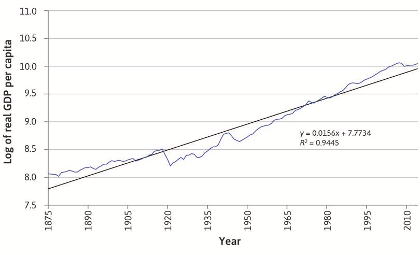
\includegraphics[width=\textwidth]{../QuestionBankImage/OUP-U13-Q04-01.png}
\answer{A}
\begin{tasks}(1)
    \task The growth of GDP in the 1950s was above the long-run average.
        \details{The slope of the blue line is steeper than that of the black line and so growth is more rapid. The fact that it lies below the black line is irrelevant.}
    \task The growth of GDP in the 1880s was above the long-run average.
        \details{The slope of the blue line is flatter than that of the black line, so the growth rate is less than the long run average. The fact that the blue line lies above the black is irrelevant.	In the figure the coefficient on x is 0.0156 and tells us the slope of the regression line (line of best fit).}
    \task If, instead, this were 0.02 the line would be flatter.
        \details{The coefficient tells us the change in the log of per capita GDP for every unit change in x where x is one year. If the coefficient were 0.2, then this would indicate that the log of per capita GDP increased each year by 2 per cent (rather than 1.56\%) and so the regression line would be steeper.}
    \task The slope of the blue line tells us the rate of growth of per capita GDP but can tell us nothing about the level.
        \details{It is correct that the slope of the blue line tells us the growth rate but each point on the blue line tells us the log of per capita GDP at that date and from the log we can calculate the actual value of GDP per capita.}
\end{tasks}

\Question (OUP-U13-Q9)
The data for Spain suggests that Okun’s Law can be written as y = -0.3147x +1.2821, where y is the change in unemployment rate and x is the GDP growth rate. What is the predicted change in unemployment if GDP grows by 2 per cent?
\answer{C}
\begin{tasks}(1)
    \task Unemployment increases by 1.9115 percentage points.
        \details{1.9115 is the value we get if we ignore the negative sign on the coefficient. (1.2821 + 0.3147(2) = 1.9115).}
    \task Unemplyoment increases by 1.2758 percentage points.
        \details{1.2758 is the value we get if we enter 0.02 for 2 per cent, when the equation requires us to enter it as a whole number. (1.2821 – 0.3147(0.02) = 1.9115.}
    \task Unemployment increases by 0.6527 percentage points.
        \details{1.2821 -0.3147(2) = 0.6527}
    \task Unemployment increases by 1.2192 percentage points.
        \details{1.2192 is the value we get if we enter the growth rate as 0.2 instead of 2. 1.2821 - 0.3147(0.2) - 1.2192}
\end{tasks}

\Question (OUP-U13-Q15)
Why is investment spending likely to be more volatile than consumption spending?
\answer{C}
\begin{tasks}(1)
    \task Because investment depends entirely on ‘animal spirits’.
        \details{It is true that he anticipated profits from investment spending depend upon a firm’s view of likely future developments and therefore upon ‘confidence’ which contains a strong psychological element. But the calculation of those likely future profits (by discounting the expected future cashflow) remains a rational exercise, albeit with some uncertainty.}
    \task Because firms cannot foresee the future.
        \details{But neither can households. Nevertheless, they try to smooth their consumption and base it upon some long-run view of what they expect to earn over a lifetime.}
    \task Because a large part of consumption spending is on items that cannot be postponed. (‘non-discretionary’) – food, heating, lighting, shelter, for example.
        \details{These items include food, heating, lighting, shelter, for example. Such spending is sometimes referred to as ‘non-discretionary’ spending.}
    \task Interest rates fluctuate.
        \details{They do, and interest rates are an important input in the investment decision. But they are relevant o consumption as well. For example, a rise in interest rates makes consuming now more ‘costly’ in relation to consuming in future because the higher interest rate generates greater income for consumption in the future period. Current consumption is likely to be reduced, rather like investment.}
\end{tasks}

\Question (OUP-U13-Q17)
Your economy is estimated to be producing about \$800bn-worth of goods and services this year. However, your official statisticians estimate that if all resources were fully-employed, it could produce about \$1000bn. The ratio 0.8 (or 80\%, $ \frac{800bn}{1000bn} $) therefore indicates:
\answer{C}
\begin{tasks}(1)
    \task The level of unemployment.
        \details{If we took the residual of 0.2 (i.e. 1 – 0.8) we would have a measure of the extent to which resources in general were underused. But ‘unemployment’ refers to the underutilisation of labour specifically. From the number 0.8 we can infer that unemployment (of labour) is likely to be positive but we cannot say more than that.}
    \task The savings ratio.
        \details{The savings ratio refers to households’ saving (non-consumption) as a fraction of their actual income. Here we have a measure of aggregate income as a fraction of potential income.}
    \task The degree of capacity utilisation.
        \details{By showing the current level of output against the maximum potential output, the degree of capacity utilisation is very useful to policymakers who may be contemplating a stimulus to the economy. It gives some indication of the size of desired stimulus.}
    \task A budget surplus.
        \details{A ‘surplus’ is involved in the sense that 0.8 shows that there is a surplus of productive capacity over what is currently being used. But the term ‘budget’ usually refers to the central government’s revenue and expenditure (and a surplus would represent an excess of revenue over expenditure). It’s also possible that a budget surplus is more likely if the economy is operating at full rather than 80\% of capacity. But the degree of capacity utilisation and a budget deficit are entirely different things’.}
\end{tasks}

\Question (OUP-U13-Q19)
In the current year, your economy is expected to make exports of \$100bn and to import \$80bn-worth of goods and services. When it comes to measuring GDP (or aggregate demand) the net effect of your external sector is to:
\answer{A}
\begin{tasks}(1)
    \task External trade contributes \$20bn.
        \details{A ‘positive trade balance’ or ‘positive net exports’ are an addition to GDP (and aggregate demand). Here the contribution is \$20bn.}
    \task External trade reduces GDP by \$20bn.
        \details{A reduction in GDP (and aggregate demand) would require negative net exports, i.e. X < M. But here the difference is positive.}
    \task We cannot tell.
        \details{Most official statistics come with a margin of error. But there’s no reason to suppose that import/export figures are particularly unreliable. There is one thing that we do not know, however. Like any autonomous addition to aggregate demand, net exports are likely to have secondary, subsequent effects. They may start by boosting aggregate demand by \$20bn but that increase may lead to further increases through a process known as the multiplier. Without knowing the value of the multiplier we cannot know the ultimate effect of net exports. We look at the multiplier process in Unit 14.}
    \task It depends on the composition of imports and exports.
        \details{The initial impact on GDP depends only on the size of the expenditure. The earnings from the sale of services, for example, are just as relevant as the earnings from goods. Of course, there will be other effects which do depend on the composition. If UK cars become very fashionable with overseas buyers, the car industry will expand and the area of its location will become more prosperous. However, if foreign cars become more fashionable in the UK, the reverse will happen.}
\end{tasks}

\Question (OUP-U13-Q13)
A temporary change in income affects the current consumption of credit-constrained households more than it does that of the unconstrained because:
\answer{B}
\begin{tasks}(1)
    \task A credit-constrained household is unlikely to have savings to fall back on.
        \details{Not necessarily. Borrowing (using credit) and saving are different things. Financial institutions may be unwilling to extend credit to certain types of household but they are unlikely to decline their savings. If credit-constrained households lack savings, it must be for some additional reason.}
    \task If the household cannot borrow, its current consumption is limited by its current income.
        \details{If it cannot borrow, then it cannot consume more than its income.}
    \task A credit-constrained household cannot foresee the future.
        \details{Foreseeing the future is difficult for everyone. It is not peculiar to credit-constrained households. The problem with credit constraints is not that they prevent one from looking ahead, but that the prevent one from taking action to deal with what one foresees.}
    \task Credit-constrained households are likely to be shortsighted.
        \details{Taking only a very short-term view is likely to tie consumption more closely to income since temporary changes in income will not be seen as temporary. But there’s no reason to suppose that this is necessarily a characteristic of credit-constrained households.}
\end{tasks}

\Question (OUP-U13-Q16)
The figure shows that total investment spending can be volatile because the interaction of individual firms’ decisions can lead to vicious (low profit) or virtuous (high profit) circles. Which of the following might encourage all firms in the economy to behave in such a way that they all increase their investment spending together?
    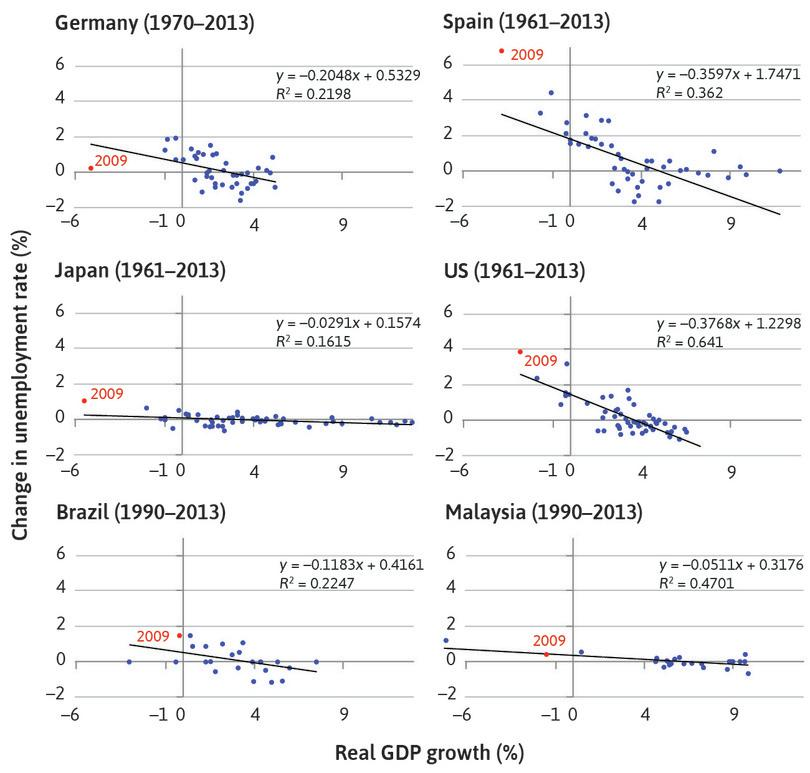
\includegraphics[width=\textwidth]{../QuestionBankImage/OUP-U13-Q7-01.jpg}

\answer{C}
\begin{tasks}(1)
    \task A fall in the exchange rate (the domestic currency becomes cheaper for foreign buyers).
        \details{This makes exports cheaper and imports dearer. Net exports are likely to increase and that will give boost to aggregate demand. But the positive effect will be limited to firms with significant exports and firms that have to buy materials from overseas will find their costs rising (and sales possibly falling).Also, fluctuations in exchange rates happen frequently. Any rise or fall is likely to be temporary. So a general boost to investment is unlikely.}
    \task A major technological breakthrough – say in batteries for electric cars.
        \details{Clearly, this is likely to encourage more investment in the automobile industry and in battery manufacture. Some firms may also recognise it as having implications for their industry even though they don’t make electric cars. But even with this ‘good news effect’ technological breakthroughs, however, general their application are unlikely to encourage all firms to expand investment simultaneously.}
    \task The use by government of fiscal policy to increase aggregate demand.
        \details{An increase in aggregate demand will encourage all firms to expect a higher demand for their products and this should have a beneficial effect on investment plans across the economy. This will be especially true if the policy is given lots of publicity and if the government’s promises are seen as credible.}
    \task Calls from government for firms to increase investment.
        \details{This is unlikely to have much effect. Firms undertake investment in order to remain competitive and/or to expand production. They do this because they see the possibility of profit and their shareholders will expect them to make the best decisions with respect to profit. Investments risky and firms are unlikely to undertake it just because governments ask them to do it. However, such encouragement might have some effect if combined with the publicity surrounding an expansionary fiscal policy.}
\end{tasks}

\Question (OUP-U14-Q3)
In the expression for aggregate consumption $C = C_0 + C_1 Y$, $ C_1 $ is known as:
\answer{D}
\begin{tasks}(1)
    \task Autonomous consumption.
        \details{‘Autonomous’ means independent of income. $ C_0 $ shows the level of consumption that does not depend upon income.}
    \task The average propensity to consume.
        \details{The average propensity to consume is given by total consumption divided by income. $ C_1 $ shows the extent to which consumption changes with income. Assuming that $ C_1 $ is less than one, the average propensity to consume will be falling as income increases even though $ C_1 $ is constant.}
    \task The multiplier.
        \details{The multiplier shows the extent to which income changes as a result of a change in autonomous spending. The formula for the (simple) multiplier is $1/(1 - C_1)$.}
    \task The marginal propensity to consume.
        \details{$ C_1 $ is the marginal propensity to consume. It normally take a value less than one, showing that an initial change in autonomous spending will initiate a series of changes of diminishing size.}
\end{tasks}

\Question (OUP-U14-Q7)
In an economy with no taxation and no external trade, the size of the multiplier depends on:
\answer{D}
\begin{tasks}(1)
    \task Investment.
        \details{In a closed economy with no government, the level of investment determines the current level of aggregate demand ($Y = C + I$).}
    \task The current level of aggregate demand.
        \details{The simple multiplier formula is $1/(1 - MPC)$, which does not depend on the level of aggregate demand ($ Y $).}
    \task Autonomous consumption.
        \details{Autonomous consumption ($ C_0 $) is the part of consumption that does not depend upon income, so it would not affect the size of the multiplier.}
    \task The marginal propensity to consume.
        \details{The simple multiplier formula is $1/(1 - MPC)$, where MPC is the marginal propensity to consume.}
\end{tasks}

\Question (OUP-U14-Q10)
In the figure shown, a fall in output is caused by a reduction in investment. Which of the following would help restore output to its original level?
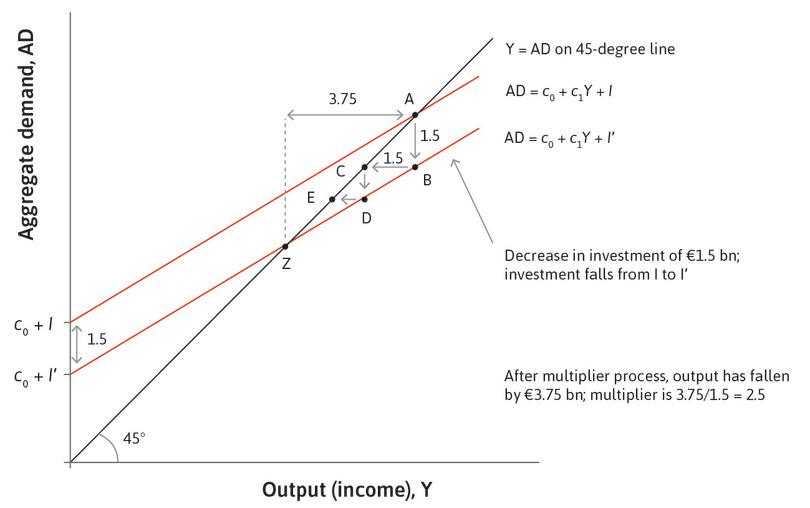
\includegraphics[width=\textwidth]{../QuestionBankImage/OUP-U14-Q10-01.jpg}
\answer{C}
\begin{tasks}(1)
    \task A reduction in autonomous consumption.
        \details{What is required is some compensating increase in aggregate demand. A reduction in autonomous consumption (the vertical axis intercept) will further reduce aggregate demand.}
    \task An increase in target wealth.
        \details{An increase in target wealth is likely to encourage households to save more, thus reducing aggregate demand.}
    \task An increase in actual wealth.
        \details{However, an increase in actual wealth may persuade them that there is less need to save. If so, consumption will increase and may compensate for the fall in investment.}
    \task A tightening of credit conditions.
        \details{A tightening of credit conditions will make borrowing more difficult, which will discourage consumption and may also encourage saving (which will also reduce consumption).}
\end{tasks}

\Question (OUP-U14-Q12)
In an economy where the MPC is 0.7, the proportional tax rate is 0.25 and the marginal propensity to import is 0.2, the multiplier will be:
\answer{C}
\begin{tasks}(1)
    \task 0.675
        \details{The value of the multiplier in this case is: 1/(1 - 0.7(0.75)) + 0.2 = 1/(1 - 0.525) + 0.2 = 1.48. 0.675 is the value of the multiplier if we omit the 1 in the numerator i.e. 0.475 + 0.2.}
    \task 2.1
        \details{The value of the multiplier in this case is: 1/(1 - 0.7(0.75)) + 0.2 = 1/(1 - 0.525) + 0.2 = 1.48. 2.1 is the value of the multiplier if we omit the marginal propensity to import.}
    \task 1.48
        \details{The value of the multiplier in this case is: 1/(1 - 0.7(0.75)) + 0.2 = 1/(1 - 0.525) + 0.2 = 1.48.}
    \task 2.35
        \details{The value of the multiplier in this case is: 1/(1 - 0.7(0.75)) + 0.2 = 1/(1 - 0.525) + 0.2 = 1.48. 2.35 is the value of the multiplier if we do the calculations in the wrong order, i.e. (1 - 0.7)0.75 + 0.2.}
\end{tasks}

\Question (OUP-U14-Q15)
The central bank announces a rise in the official interest rate to reduce the rate of inflation. Looking at the figure shown, ceteris paribus, the aggregate investment function in these circumstances is likely to:

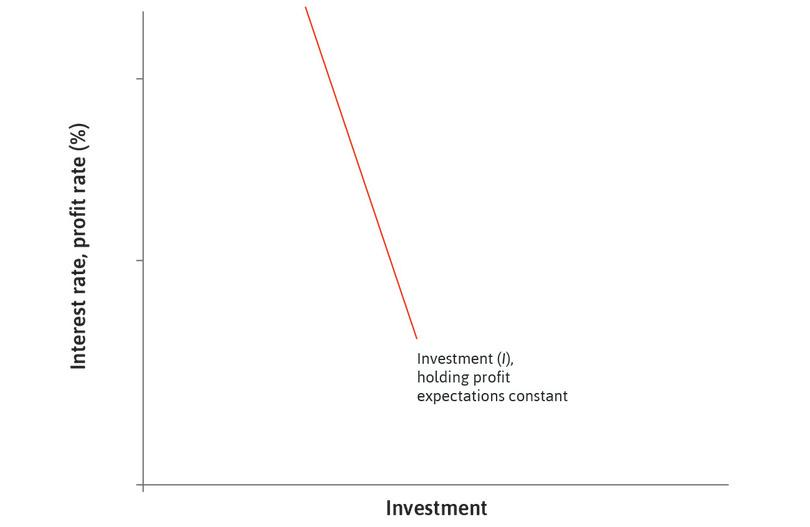
\includegraphics[width=\textwidth]{../QuestionBankImage/OUP-U14-Q15-01.jpg}
\answer{D}
\begin{tasks}(1)
    \task Become flatter.
        \details{The aggregate investment function shows the relationship between investment spending and the interest rate, ceteris paribus. A rise in the official interest rate moves us up along the investment function, indicating a fall in investment. There is no need for the investment function itself to change.}
    \task Become steeper.
        \details{Because we are dealing with a change in a variable on one of the axes, there is no need for the function itself to change. This will happen only if there is a change in some other relevant variable, not shown in the diagram.}
    \task Shift to the left.
        \details{Because we are dealing with a change in a variable on one of the axes, there is no need for the function itself to change. This will happen only if there is a change in some other relevant variable, not shown in the diagram.}
    \task Remain unchanged.
        \details{A rise in the official interest rate moves us up along the investment function, indicating a fall in investment. There is no need for the investment function itself to change.}
\end{tasks}

\Question (OUP-U14-Q22)
Cuts in public expenditure do not guarantee a reduction in the government’s deficit because:
\answer{B}
\begin{tasks}(1)
    \task Firms will try to pay less tax.
        \details{Firms (and households) may try to minimise their tax liabilities, but there is no reason to suppose that their attempts to do this are directly related to the level of government spending.}
    \task Aggregate demand will fall, reducing government revenue.
        \details{The cuts in public spending constitute a reduction in the autonomous components of aggregate demand. Through the multiplier, we must expect a fall in aggregate demand somewhat larger than the initial cut in public spending. With the fall in aggregate demand, output, and employment, there will be a fall in government revenue as fewer workers pay tax and firms pay less tax on their lower profits.}
    \task Aggregate demand falls, and firms invest less.
        \details{Aggregate demand will fall and firms may decide to invest less if they see this reduction in aggregate demand as a condition that is likely to persist, but the reduction in investment has no direct connection to the government’s revenue.}
    \task There is a fall in autonomous consumption.
        \details{There is no reason to expect a fall in autonomous consumption. Aggregate demand will fall, meaning that income will fall and there may be some reduction in consumer spending (the basis of the multiplier effect). But this will be consumer spending that is related to income, not autonomous consumption ($ C_1 $ not $ C_0 $).}
\end{tasks}

\Question (OUP-U14-Q16)
The figure shows a downward shift of the aggregate demand curve, reducing the level of output from A to Z. Suppose that we begin again at A and that this is a full-employment level of output. An increase in aggregate demand in these circumstances will most likely cause:

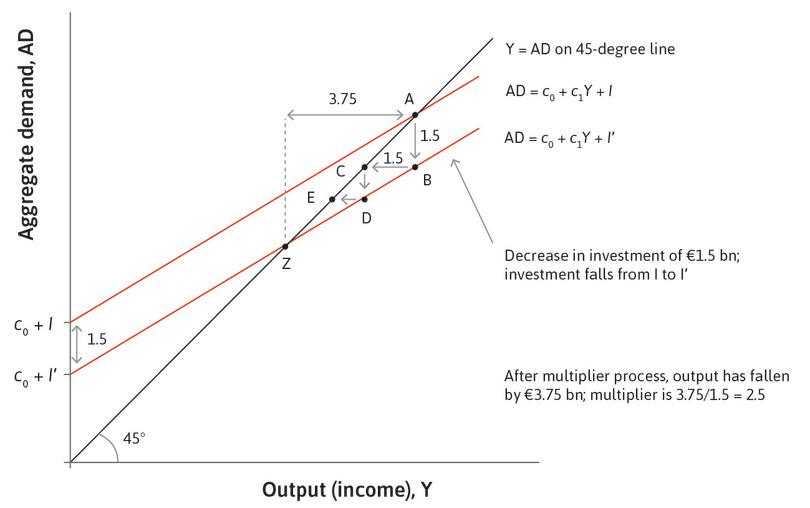
\includegraphics[width=\textwidth]{../QuestionBankImage/OUP-U14-Q10-01.jpg}
\answer{D}

\begin{tasks}(1)
    \task An increase in employment.
        \details{If the economy is producing a full employment level of output, an increase in aggregate demand cannot create more employment. It may create more jobs in one industry at the expense of another as firms compete with each other to attract more workers, but there cannot be an overall increase in employment.}
    \task A fall in wages.
        \details{The increase in aggregate demand will probably cause firms to compete against each other in a self-defeating attempt to attract more workers. This will involve higher nominal wages, but the real wage will be unchanged as firms raise prices to cover the higher nominal wages.}
    \task An increase in output.
        \details{At full employment, an increase in aggregate demand cannot produce additional output.}
    \task A rise in the general level of prices.
        \details{Attempts to increase aggregate demand when the economy is already at full employment will almost certainly cause a rise in the general price level.}
\end{tasks}

\Question (OUP-U15-Q2)
Which of the following is a definite consequence of a high inflation rate?
\answer{D}
\begin{tasks}(1)
    \task It reduces everyone’s real wealth and real income.
        \details{Inflation is unlikely to reduce everyone’s real income and wealth. The first depends upon the composition of one’s wealth. Some assets, especially real assets, can rise in price along with inflation. In the UK, house prices have often risen faster than inflation. Likewise, protecting one’s real income from inflation depends on one’s ability to bargain for a money wage increase. Depending on these conditions, some people will be losers but some may possibly benefit from inflation. The fact that who wins and who loses is something of a lottery is sometimes given as a reason for objecting to inflation.}
    \task It makes borrowing more expensive.
        \details{The cost of borrowing depends upon the real rate of interest, which is the nominal rate minus the rate of inflation. Inflation will make borrowing cheaper if the nominal rate of interest does not adjust sufficiently.}
    \task It makes poor people worse off.
        \details{This is not an ineoutcome. It depends on whether their nominal incomes and their assets keep pace with the rising price level.}
    \task It can distort price signals.
        \details{A change in price is an important signal in market economies. It can signal the need to buy more or less, supply more or less, and so on. If prices are generally rising, it can be difficult to know what an individual price increase means. Does it mean increasing scarcity, in which case some reallocation decision is required, or it is just part of the inflationary process? This can be a serious problem if inflation is running at a high rate, and especially if the rate is frequently changing.}
\end{tasks}

\Question (OUP-U15-Q11)
Suppose that the bargaining power of workers rises relative to that of employers because government legislation improves the security of employment. In terms of the wage-setting/price-setting model shown in the figure:

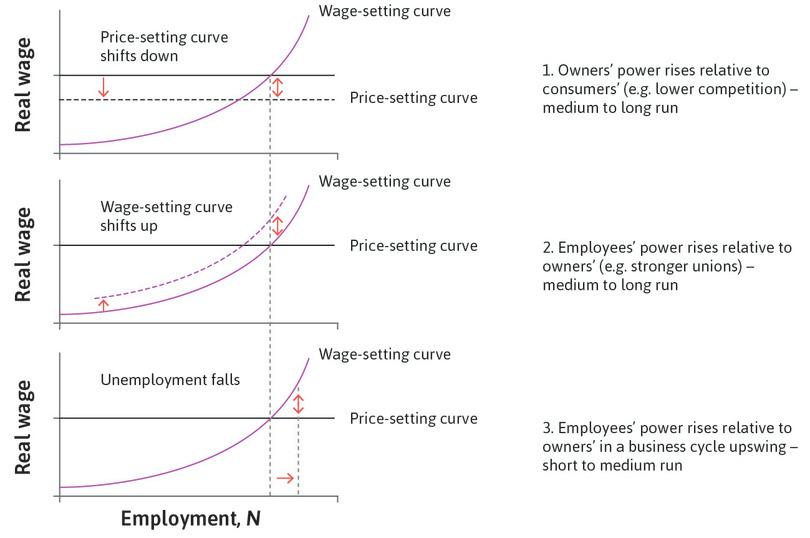
\includegraphics[width=\textwidth]{../QuestionBankImage/OUP-U15-Q11-01.jpg}
\answer{B}
\begin{tasks}(1)
    \task We move along the wage-setting curve, to the right.
        \details{No. A movement along a given wage-setting curve would require a change in the level of employment, since the diagram shows how the workers’ desired real wage varies with the level of employment.}
    \task The wage-setting curve moves up.
        \details{Correct. The wage-setting curve shifts up because the improved security of employment encourages workers to seek higher wages at every level of employment.}
    \task The wage-setting curve moves down.
        \details{No. This would suggest that the legislation encouraged workers to settle for lower wages at every level of employment.}
    \task The wage-setting curve becomes flatter.
        \details{This would suggest that workers were becoming less concerned about higher real wages as employment expands, which is not guaranteed by a rise in their bargaining power.}
\end{tasks}


\Question (OUP-U15-Q20)
Assume that a bargaining gap remains constant at 1 per cent. The rate of inflation in future years will:
\answer{C}
\begin{tasks}(1)
    \task Remain constant at 1 per cent per year.
        \details{No. If there is a positive bargaining gap, there will be upward pressure on prices. This will be added to any existing rate of inflation, so the rate of inflation must accelerate.}
    \task Remain unchanged.
        \details{No. For the same reason, inflation must be accelerating.}
    \task Accelerate by 1 per cent per year.
        \details{Correct. If the bargaining gap is constant at 1 per cent, this will be added to the rate of inflation each year and so inflation will increase (accelerate) by 1 per cent per year.}
    \task Settle at 1 per cent.
        \details{No. So long as there is a bargaining gap, inflation cannot settle at any level. It must be accelerating or decelerating.}
\end{tasks}

\Question (OUP-U15-Q22)
Assume that the central bank has an inflation target of 2\% per year but inflation is currently running at 4\%. The nominal policy (interest) rate is currently 5\%. The central bank needs to create a negative bargaining gap and estimates that the real policy rate required to achieve this is 3\%. Consequently it needs to set the nominal policy rate at:
\answer{B}
\begin{tasks}(1)
    \task 6\%.
        \details{No. If inflation is running at 4\% and the real rate needs to be 3\%, then according to the Fisher equation, the nominal rate needs to be 4\% + 3\% = 7\%.}
    \task 7\%.
        \details{According to the Fisher equation, 7\% is the required nominal rate.}
    \task 8\%.
        \details{No. If inflation is running at 4\% and the real rate needs to be 3\%, then according to the Fisher equation, the nominal rate needs to be 4\% + 3\% = 7\%.}
    \task 4\%.
        \details{No. The required rate is 4 + 3 = 7\%.}
\end{tasks}

\Question (OUP-U15-Q25)
It is often said that independent central banks are more likely to run a successful monetary policy than governments because their commitment to low inflation is more ‘credible’ than government promises. One reason for this is that:
\answer{D}
\begin{tasks}(1)
    \task Independent central banks are better at economic forecasting.
        \details{There is no reason to suppose that independent central banks are systematically better at forecasting than ministries of finance or private firms.}
    \task People who work in central banks have a strong dislike of inflation.
        \details{It may be possible that people who occupy senior positions in central banks are more inflation-averse than politicians or even than members of the public. If this is true, then they may be tempted to run monetary policy in their own interests and therefore with a low inflation bias. But there is no evidence for this and it is difficult to see why there would be this systematic bias.}
    \task Central banks can set interest rates.
        \details{It is true that central banks can set interest rates. In fact it is only a central bank that can impose a particular interest rate on the financial system. But the power to set the interest rate is a different issue from deciding what rate to set. It is the latter that has been moved from governments to independent central banks in recent years. It would be perfectly possible to return the decision-making to government, even though the central bank would still have to impose the rate.}
    \task Central banks are less subject to political pressures (e.g. for lower unemployment) than governments.
        \details{The argument for putting the decision in the hands of an independent central bank is based upon the view that central banks face fewer conflicts of interest, because they are not subject to political pressures. If inflation requires a very high (and unpopular) rate of interest, this is less of a problem for central banks than for governments whose electors may be more concerned about jobs.}
\end{tasks}

\Question (OUP-U15-Q18)
The main weakness of the original Phillips curve is that it ignored:
\answer{D}
\begin{tasks}(1)
    \task Time.
        \details{It didn’t ignore time; Phillips used data from 1861 to 1957. The problem was that the data for this period was misleading as a guide to the post-1957 period.}
    \task Household preferences.
        \details{There was no issue regarding household preferences.}
    \task Policymaker preferences.
        \details{There was no problem with regard to policymaker preferences, except that the original Phillips curve suggested that the feasible combinations were durable.}
    \task Expectations.
        \details{Correct. The problem was expectations. The original Phillips curve was based upon data drawn from a period when inflation was generally very low (excluding the two world wars). Therefore, in the process of wage bargaining, the future expected rate of inflation was not a major factor. In more inflationary times (1960 onwards) it was inevitable that whatever the level of unemployment and the size of the bargaining gap, workers would also be trying to take account of what they expected inflation to be, guided by the most recent rate.}
\end{tasks}



\Question (OUP-U15-Q25)
It is often said that independent central banks are more likely to run a successful monetary policy than governments because their commitment to low inflation is more ‘credible’ than government promises. One reason for this is that:
\answer{D}
\begin{tasks}(1)
    \task Independent central banks are better at economic forecasting.
        \details{There is no reason to suppose that independent central banks are systematically better at forecasting than ministries of finance or private firms.}
    \task People who work in central banks have a strong dislike of inflation.
        \details{It may be possible that people who occupy senior positions in central banks are more inflation-averse than politicians or even than members of the public. If this is true, then they may be tempted to run monetary policy in their own interests and therefore with a low inflation bias. But there is no evidence for this and it is difficult to see why there would be this systematic bias.}
    \task Central banks can set interest rates.
        \details{It is true that central banks can set interest rates. In fact it is only a central bank that can impose a particular interest rate on the financial system. But the power to set the interest rate is a different issue from deciding what rate to set. It is the latter that has been moved from governments to independent central banks in recent years. It would be perfectly possible to return the decision-making to government, even though the central bank would still have to impose the rate.}
    \task Central banks are less subject to political pressures (e.g. for lower unemployment) than governments.
        \details{The argument for putting the decision in the hands of an independent central bank is based upon the view that central banks face fewer conflicts of interest, because they are not subject to political pressures. If inflation requires a very high (and unpopular) rate of interest, this is less of a problem for central banks than for governments whose electors may be more concerned about jobs.}
\end{tasks}

\Question (OUP-U16-Q4)
In the short run, successive additions to capital produce smaller and smaller increases in output. Which of the following statement(s) could explain why GDP nevertheless continues to rise In the long run?
\answer{D}
\begin{tasks}(1)
    \task Workers work harder.
        \details{Incorrect. Worker effort is not directly related to the state of technology. Equipping workers with the latest technology may raise their morale and encourage them to work harder if they see the new technology as a vote of confidence from the firms’ owners. On the other hand, knowing that the new technology makes them more productive, they may be tempted to work less hard in order to produce the same as before.}
    \task Government policy encourages economic growth.
        \details{Incorrect. Generally speaking, governments tend to favour economic growth. But the mere fact that governments prefer growth to stagnation does not make it happen.}
    \task Economies benefit from economies of scale.
        \details{Incorrect. Individual firms may enjoy economies of scale, meaning that the unit cost of production falls as output increases. But true economies of scale must come solely from increasing the volume of production. Everything else, including the capital stock, should remain constant.}
    \task New capital equipment incorporates the latest technological developments.
        \details{Correct. In the short run, the additions to capital consist of the same kind of equipment as earlier additions to the capital stock. Eventually, ‘more of the same’ type may still increase the level of output, but at a diminishing rate. But once we relax the short-run constraint, successive additions to capital cease to be ‘more of the same’ and rather will consist of more and more productive equipment.}
\end{tasks}



\Question (OUP-U16-Q8)
The relationship between the unemployment rate and the job vacancy rate (each expressed as a fraction of the labour force) is known as:
\answer{D}
\begin{tasks}(1)
    \task The Phillips curve.
        \details{Incorrect. The Phillips curve plots the rate of growth of wages against the level of unemployment.}
    \task The labour demand curve.
        \details{Incorrect. The labour demand curve shows the quantity of labour demanded (by employers) at each level of real wages.}
    \task The wage-setting curve.
        \details{Incorrect. The wage-setting curve shows the amount of labour that workers are willing to supply at each level of real wages.}
    \task The Beveridge curve.
        \details{Correct. The Beveridge curve shows the relationship between the unemployment rate and the job vacancy rate.}
\end{tasks}




\Question (OUP-U16-Q11)
The profit-maximising mark-up declines as the number of firms increases. This is because:
\answer{D}
\begin{tasks}(1)
    \task The greater the number of firms, the more market power they each have.
        \details{Incorrect. The greater the number of firms, the less market power any one firm is likely to have.}
    \task Too many firms means diseconomies of scale.
        \details{Incorrect: Economies or diseconomies of scale occur within an individual firm. It has nothing to do with the number of firms.}
    \task The lower the individual mark-up, the more firms can share in the profits.
        \details{Incorrect. This would be true if the total amount of profit was fixed, but the total amount of profit is likely to vary positively with the number of firms.}
    \task The larger the number of firms, the more competitive the system is likely to be.
        \details{Correct. The larger the number of firms, the more competitive the system is likely to be, and each firm will be obliged to accept the minimum level of profit necessary to keep it functioning.}
\end{tasks}



\Question (OUP-U16-Q14)
The widespread introduction of new technology into an economy takes time. The length of time between first appearance and general acceptance is known as:
\answer{D}
\begin{tasks}(1)
    \task The innovation lag.
        \details{Incorrect. This is a sensible label that could be used to describe the lag between the development of a new technology and its application, but it is not used for this purpose.}
    \task The time gap.
        \details{Incorrect: The term ‘time gap’ is very widely used to describe the time between two events or developments, but it does not refer specifically to the delay here.}
    \task The knowledge lag.
        \details{Incorrect. This could refer to a number of situations but does not relate specifically to innovation.}
    \task The diffusion gap.
        \details{Correct. The ‘diffusion gap’ refers to the length of time required for a technological innovation to become ‘diffused’ throughout the economy.}
\end{tasks}



\Question (OUP-U16-Q16)
As a result of the diffusion of new technology, in the long run we would normally expect:
\answer{D}
\begin{tasks}(1)
    \task The price-setting curve to shift downwards.
        \details{Incorrect. The new technology increases output per worker. There is no reason to suppose that the share of total output required by firms as profit has changed. Therefore the price-setting curve shifts upwards to maintain the firms’ share of total output.}
    \task The price-setting curve to slope downward more steeply.
        \details{Incorrect. The price-setting curve is a horizontal line showing the real wage that firms are willing to pay in order to deliver the desired profit share (= output per worker – real wage).}
    \task An increase in unemployment.
        \details{Incorrect. There may be some unemployment in the short run if some workers are unable to use the new technology, but the lasting effect depends on what happens to the wage-setting curve. If it remains unchanged, there will be a fall in unemployment, rather than an increase.}
    \task The price-setting curve to shift upwards.
        \details{Correct. The new technology increases output per worker. There is no reason to suppose that the share of total output required by firms as profit has changed. Therefore the price-setting curve shifts upwards to maintain the firms’ share of total output.}
\end{tasks}




\Question (OUP-U16-Q20)
The figure shows long-run unemployment and real wage growth across the OECD. The rays drawn from the origin are described as ‘indifference curves’. This is because:
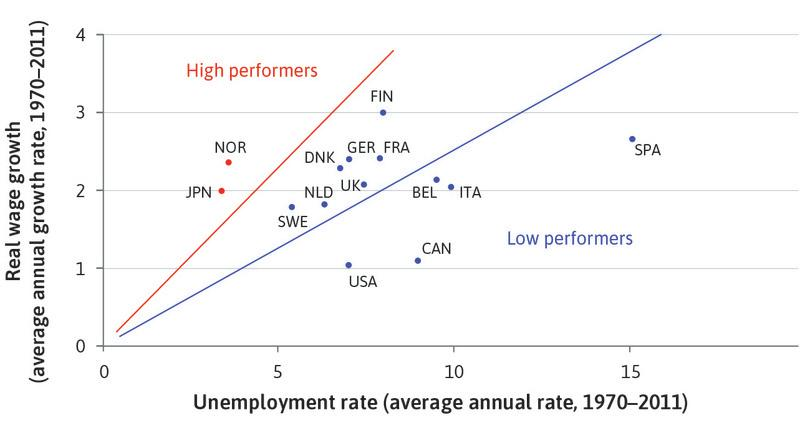
\includegraphics[width=\textwidth]{../QuestionBankImage/OUP-U16-Q20-01.jpg}
\answer{D}
\begin{tasks}(1)
    \task They show that people are indifferent to levels of unemployment.
        \details{Incorrect. ‘Indifferent to levels of unemployment’ would mean that they did not care about the level of unemployment. But an upward-sloping indifference curve means that people are prepared to accept higher unemployment only if real wages grow more rapidly.}
    \task They show a trade-off between unemployment and real wage growth.
        \details{Incorrect. A ‘trade-off’ means that more of something requires less of something else. But here, people are indifferent between combinations of high unemployment and high real wage growth, and low unemployment/low real wage growth. Therefore there is no trade-off involved.}
    \task They show that real wage growth and low unemployment go together.
        \details{`Incorrect. They show that real wage growth and high unemployment go together.}
    \task Each ray shows the combinations of unemployment and real wage growth that correspond to the same 'utility'.
        \details{An indifference curve shows combinations of two variables that give equal satisfaction. In the figure we can see that people can be equally happy with high or low unemployment, provided that higher unemployment is accompanied by higher real wage growth.}
\end{tasks}



\Question (OUP-U16-Q22)
Looking at the figure shown, if it were the case that countries with strong trade unions also experienced high unemployment rates, we would expect the data points to be:
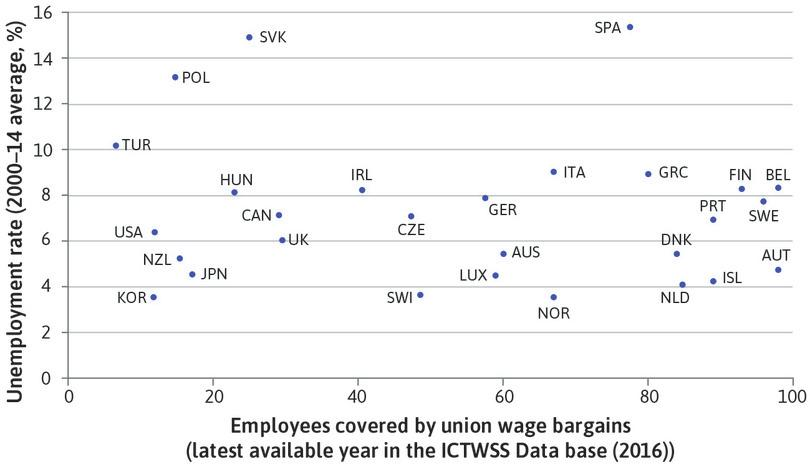
\includegraphics[width=\textwidth]{../QuestionBankImage/OUP-U16-Q22-01.jpg}
\answer{C}
\begin{tasks}(1)
    \task Clustered around a horizontal line.
        \details{Incorrect. If the data points lay close to a horizontal line, this would tell us that the level of unemployment (at which the line were drawn) was consistent with any level of trade union membership. There is no apparent connection between trade union strength and unemployment.}
    \task Clustered around a downward-sloping line.
        \details{Incorrect. If the points were clustered around a downward-sloping line, this would tell us that there might be some connection between unemployment and trade union strength, but the relationship is negative. Trade union strength is associated with low unemployment.}
    \task Clustered around an upward-sloping line.
        \details{Correct. If the points were clustered around an upward-sloping line, this would tell us that there might be some positive connection between unemployment and trade union strength. Trade union strength appears to be linked to high unemployment.}
    \task More randomly dispersed than they are.
        \details{Incorrect. In the figure, the data points are widely dispersed. There is no obvious relation between trade union strength and unemployment. If the data points were more randomly dispersed than they already are, this would make the lack of a connection even clearer.}
\end{tasks}

\Question (ECO-U16-Q7)
Figure 16.9b depicts the long-run adjustment process in the labour market after technological progress. Based on this information, which of the following statements is correct?
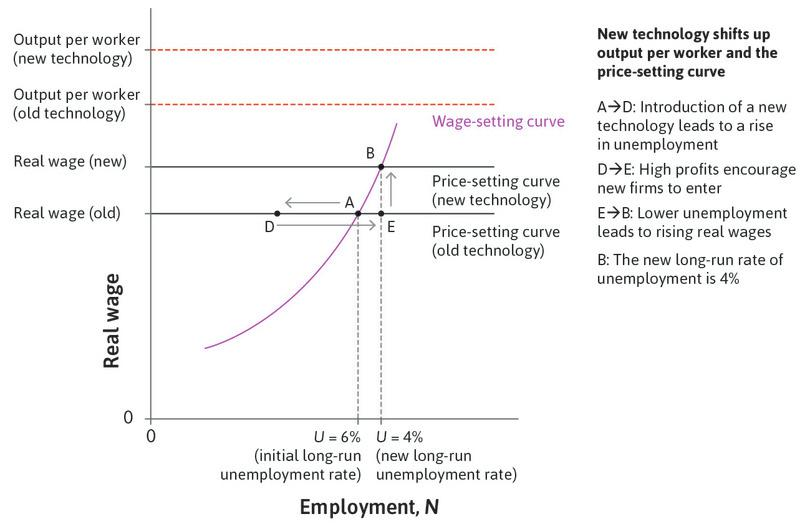
\includegraphics[width=\textwidth]{../QuestionBankImage/ECO-U16-Q7-01.jpg}
\answer{C}
\begin{tasks}(1)
    \task The new technology does not cause any increase in unemployment, either in the short run or in the long run.
        \details{In the short-run, initially there is a displacement of some workers from their jobs, which increases unemployment, as shown by the movement from point A to point D.}
    \task At D firms increase investment, and hence employment, due to the large gap between the real wage paid and the workers’ wage-setting curve.
        \details{Firms increase investment due to the large gap between the old real wage (solid line) and the new output per worker (dashed line), which implies higher profits.}
    \task Lower unemployment at E implies a higher wage required to induce workers to exert high effort, resulting in the higher real wage at B.
        \details{E is below the wage-setting curve so workers need a higher wage to be induced to work.}
    \task The adjustment from equilibrium A to the new equilibrium at B is immediate.
        \details{The adjustment to the new equilibrium requires entry of new firms, which can take a substantial amount of time.}
\end{tasks}




\Question (OUP-U16-Q6)
Last year, an economy had 1m registered unemployed and a labour force of 20m. Official statistics forecast a level of unemployment of 0.8m by the year’s end while the size of the labour force remains unchanged. If this happens then the unemployment rate will have:
\answer{B}
\begin{tasks}(1)
    \task Risen by 0.2m.
        \details{Incorrect. The level of unemployment has fallen by 0.2m. If the labour force is constant, then the rate of unemployment must also have fallen.}
    \task Fallen from 5 per cent to 4 per cent.
        \details{Correct. The unemployment rate has fallen from 1/20 (= 5\%) to 0.8/20 (= 4\%).}
    \task Fallen by 0.2m.
        \details{Incorrect. The level of unemployment has fallen by 0.2m, but the question asks about the rate.}
    \task Fallen by 0.2 per cent.
        \details{Incorrect. The level of unemployment has fallen by 0.2m but 0.2m is 1 per cent of 2m.}
\end{tasks}

\Question (OUP-U17-Q4)
The figure shows that central banks reduced interest rates more sharply and kept them lower after the 2008 crisis than they did in the 1930s. But the figure shows nominal interest rates. Bearing in mind that inflation was slightly negative in the early 1930s and approximately zero from 2009, which of the following statements could be true about monetary policy after 1929 and after 2008?
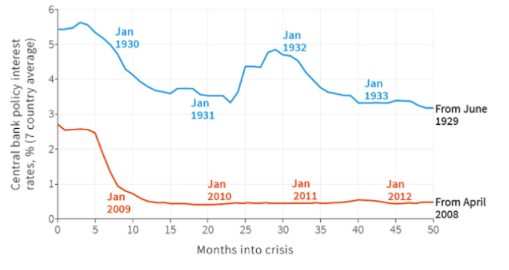
\includegraphics[width=\textwidth]{../QuestionBankImage/OUP-U17-Q4-01.png}
\answer{D}
\begin{tasks}(1)
    \task It is real (not nominal) rates that matter, so the figure tells us nothing useful.
        \details{The real interest rate is the nominal rate minus the rate of inflation. Given that you know inflation is negative in the early period and zero in the later period, you can use the figure to deduce approximate real interest rates and make some statements about monetary policy.}
    \task Since inflation is roughly zero, the nominal and real rates are the same in both periods.
        \details{This is correct for the later period, but what about the real rate in the earlier period?}
    \task When we account for inflation, there is little difference in the stance of monetary policy in the two periods.
        \details{Look again at the formula for the real interest rate. What is the real interest rate in the earlier period?}
    \task When we consider real interest rates, monetary policy was even tighter in the 1930s compared with 2008 onwards.
        \details{Given that prices were falling in the early 1930s, the real rate is even higher than the nominal rate shown in the figure. In the later period, with stable prices, the real and nominal rates are the same. So when we look at real rates, the gap between the two periods is even larger than it appears in the figure.}
\end{tasks}



\Question (OUP-U17-Q9)
In the diagram shown, demand for the industry’s goods falls from A to B. In the new equilibrium at C, individual firms are now receiving lower revenue. If they try to restore their earnings by producing more, which of the following is likely to happen in the short run?
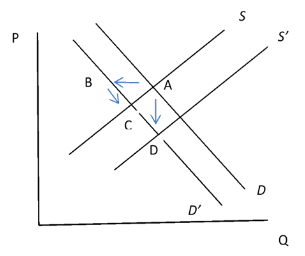
\includegraphics[width=\textwidth]{../QuestionBankImage/OUP-U17-Q9-01.png}
\answer{B}
\begin{tasks}(1)
    \task They will not be able to sell the additional output, so the market remains at C.
        \details{This assumes that the increase in supply has no effect on the equilibrium price and quantity, which seems unlikely.	The increase in supply will drive prices down even further (for example, to point D).}
    \task Producers face a catastrophic fall in prices, partly of their own making.
        \details{We can imagine a shift in the supply curve, assuming that in the short run firms are prepared to sell at prices that ignore costs of production. Doing so is unsustainable, and at point D many firms will go out of business. Supply will fall and prices will recover.}
    \task We cannot predict what will happen.
        \details{There may be some uncertainty regarding the exact quantity sold in the short run. However, provided the supply and demand schedules are based on firm evidence, we know that an increase in production must drive the price down further, with potentially catastrophic results. We can also make predictions based on similar events that happened in the past (in this case, the US farmers in the Great Depression).}
    \task The direction of price and quantity changes depends on the elasticity of demand.
        \details{It is quite correct that the actual size of the price and quantity movements depends upon the elasticity (or slope) of both the demand and supply curves. However, if the demand curve has a negative slope and the supply curve has a positive slope, we can be sure of the directions of adjustment.}
\end{tasks}




\Question (OUP-U17-Q11)
You are given the following information about the short-term nominal interest rate and the rate of inflation over a period of 8 years. In which year was the real rate of interest at its maximum and in which years might we regard monetary policy as having been expansionary?
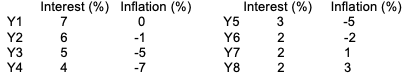
\includegraphics[width=\textwidth]{../QuestionBankImage/OUP-U17-Q11-01.png}
\answer{B}
\begin{tasks}(1)
    \task The real rate is at its maximum in Y4, but monetary policy is expansionary in all years since the rate of interest is falling.
        \details{The first part is correct. The real rate in Y4 is 11\% (= 4 - -7). However, the real rate has been rising since Y1 (7\%, 7\%, 10\%, 11\%) in spite of reductions in the nominal rate.	The real rate is at its maximum in Y4. It starts to fall in Y5 and falls below the Y1 rate in Y6.}
    \task Y6 is the earliest point at which we can describe monetary policy as expansionary.
        \details{The real rate is at its maximum in Y4. In spite of cuts to the nominal rate from Y1, the real rate does not fall below the rate in Y1 until we get to Y6 (= 4\%). The real rate does not turn negative until Y8.	The real rate is at its maximum in Y1 (= 7\%).}
    \task It only becomes negative in Y8, which is the earliest that we can describe policy as expansionary.
        \details{The real rate is higher in Y4 at 11\% (= 4 - -7). It is true that the real rate only becomes negative in Y8, but it falls below its initial (Y1) rate in Y6. We could argue that this reduction below the starting rate is where the expansionary policy starts.}
    \task The real rate is at its maximum in Y1 (=7\%) and monetary policy becomes expansionary in Y3 when the real rate falls to zero (= 5 - 5).
        \details{The real rate is at its maximum in Y4 at 11\% (= 4 - -7). In Y3, the real rate is actually 10\% (= 5 - -5). Note: we need to subtract a negative inflation rate.}
\end{tasks}



\Question (OUP-U17-Q20)
According to the original Phillips curve (Unit 15), higher inflation is associated with lower unemployment. The term ‘stagflation’ was coined to describe the unusual situation in the 1970s where unemployment and inflation both rose together. Which of the following best summarises the underlying causes?
\answer{D}
\begin{tasks}(1)
    \task Lower profits and a reduced rate of net investment meant a slower increase in productivity.
        \details{The Phillips curve says nothing about profits, investment, or productivity. These events may be involved in the change, but the answer does not explain how they contributed to high unemployment and inflation.}
    \task The lower growth of productivity meant a slower growth in the real wage and in the upward movement of the price-setting curve.
        \details{This may be correct, but does not explain the increase in unemployment.	The lower productivity growth of productivity meant slower real wage growth and a smaller upward movement of the price-setting curve. At the same time, the nature of industrial relations meant that the wage-setting curve also shifted upwards.}
    \task The result is that the wage and price-setting curves intersect at a lower employment (higher unemployment) rate than before.
        \details{This explains the higher levels of unemployment in the 1970s but not the higher rates of inflation that went with it.	The lower growth of productivity meant a slower growth in the real wage and in the upward movement of the price-setting curve. In addition, the succession of oil price shocks caused a rise in prices that firms could only partially pass on. This also ate into profits, reducing further the upward movement of the price-setting curve.}
    \task It also led people, workers especially, to expect inflation and therefore to build it into wage settlements.
        \details{This explains both the increase in unemployment and inflation.}
\end{tasks}



\Question (OUP-U17-Q22)
The leverage ratio is defined as total assets/equity. Assume that a household’s sole asset is a house worth \$190,000, which it has bought with a mortgage loan of \$180,000. What is the value of the leverage ratio, and what happens to the ratio if the house value falls to \$185,000?
\answer{A}
\begin{tasks}(1)
    \task 19; 37.
        \details{The ratio begins at 19 (= 190/10) and rises to 37 (185/5) as the value falls. Notice how the small change in the value dramatically changes the ratio.}
    \task 19; 18.5.
        \details{The ratio begins at 19 (= 190/10) and rises to 37 (185/5) as the value falls. Remember, the ratio divides the value of the asset by the value of equity. As the value falls, both the value and the equity fall.}
    \task 0.053; 0.027.
        \details{These are the inverse of the correct values. Remember, the leverage ratio divides the asset value by the equity value, not the other way round.}
    \task 19; 13.
        \details{19 is correct for the initial value but 13 is the value of the ratio if the price increases by \$5,000 (to \$195,000) instead of falling to \$185,000. Note again though how the small change in value has a large effect on the ratio.}
\end{tasks}



\Question (TEA-U17-Q1)
Herbert Hoover was the US President between 1929 and 1933. During this time: (1) President Hoover advocated a balanced budget which remained within the range of -0.6\% to +0.8\% of GNP in 1929-31, (2) Output was 20\% below the full employment level in 1931, (3) The short-term nominal interest rate fell from 5.8\% in 1929 to 1.7\% in 1933, (4) The CPI decreased from -2.7\% in 1930 to -10.3\% in 1932 and (5) The US remained on the gold standard while the UK abandoned the regime in 1931. hich of the following statements regarding this period is correct?
\answer{B}
\begin{tasks}(1)
    \task The government’s balanced budget contributed to the stabilisation of economic activity.
        \details{Given that the output was 20\% below the full employment level in 1931 there must have been a large decline in tax revenues. Therefore a balanced budget would have meant a large cyclically adjusted surplus. Thus in reality there was a large fiscal contraction.}
    \task Despite the cut in the nominal interest rate, monetary policy was contractionary during this period.
        \details{Even though the nominal interest rate fell, the real interest rate was rising because prices were falling.}
    \task The cut in the nominal interest rate was possible due to the US remaining in the gold standard.
        \details{Remaining in the gold standard meant that the nominal interest rate needed to be kept high relative to other countries in order to attract an inflow (or prevent the outflow) of gold. The nominal interest rate was cut to close to zero once the US left the gold standard in 1933.}
    \task The fact that the UK left the gold standard made it easier for the US to remain in the gold standard.
        \details{Once the UK left the gold standard there were expectations that the US would also leave, leading to a large outflow of gold. This made it difficult for the US to remain in the gold standard.}
\end{tasks}



\Question (OUP-U17-Q13)
Imagine that you are responsible for policymaking in an economy that is experiencing a deep recession. You and your colleagues announce a number of measures (like those in Roosevelt’s ‘New Deal’) that you tell everyone will boost demand and output. Why does it matter whether the public believes your announcement?
\answer{B}
\begin{tasks}(1)
    \task It does not. If the measures are appropriate, aggregate demand will increase, regardless of what anyone thinks.
        \details{Remember that lots of spending decisions have a forward-looking focus. This is especially true of firms’ investment plans but also of households’ decisions to buy durable goods. This immediately makes expectations relevant. If people believe that aggregate demand is going to increase (output rise, unemployment fall), they will feel more confident, spend more, and give a further boost to aggregate demand.}
    \task People will feel more confident about the future and increase their spending, which will reinforce the actions of government.
        \details{If people believe your announcement, they will feel more confident and may bring forward their spending plans or be encouraged to invest more. This helps to make your announcement something of a ‘self-fulfilling prophecy’. It is also similar to the positive feedback mechanism we discussed earlier in this unit.	If they really believe that you are going to increase government spending, they may worry that taxes will have to rise in future. They will reduce their spending in order to save more for the future tax demands, which will undermine your strategy.}
    \task It might be better if they simply ignored your promises.
        \details{It is always possible that people react adversely to policy announcements, especially if they do not understand them. This is why ‘presentation’ is often important and why Roosevelt stressed the need to be bold. In this case, to think that increasing public spending in a recession is a bad idea, people have to ignore the fact that such spending is likely to boost output, employment, and incomes, which is unlikely.}
    \task You are more likely to be re-elected if people believe that you tried to do something.
        \details{It is possible for policymakers to make these announcements and launch these plans in order to get re-elected. However, this is a dangerous strategy, because re-election is unlikely if these plans turned out to be a disaster. If people’s confidence in you as a policymaker matters, it must be because their confidence helps you bring about some improvement in the economy.}
\end{tasks}



\Question (OUP-U17-Q24)
It is well known that financial transactions frequently involve asymmetric information, because one party to the deal (usually the borrower) has better information about the risk and return to which the borrowed funds will be exposed than the other party (typically the lender). How does the concept of asymmetric information help us understand the particular events described in Section 17.11 (The role of banks in the crisis)?
\answer{C}
\begin{tasks}(1)
    \task Banks were reluctant to lend to households and firms because they did not know the risks involved.
        \details{This is not a special feature of the credit crunch. It is part of the general problem of asymmetric information and banks usually make credit assessments under conditions of normal uncertainty and ignorance. The problems referred to in the text concern the interbank market – the market through which banks lend to each other for very short periods – sometimes as short as overnight.}
    \task Central banks were reluctant to provide liquidity because they could not make an accurate assessment of which banks were solvent.
        \details{This was certainly a worry, but central banks reacted by relaxing their conditions, cutting the official interest rate, and trying to persuade banks to borrow. However, banks were reluctant to borrow from the central bank, probably because they feared that in the nervous atmosphere of the time, news that they had borrowed from the central bank would cause a panic amongst depositors.}
    \task In the credit crunch, banks were reluctant to lend to each other because they knew that risk was widespread because of large holdings of financial assets that were hard to value, and whose distribution amongst banks was unknown.
        \details{Banks knew the risk of default was generally high but could not pin down the risk for any individual bank. The probability of default could not be estimated and so the normal pricing formula (shown in the text) could not be used. This meant the safest strategy was not to lend at all. The interbank market seized up.}
    \task Households were reluctant to lend to banks because they could not assess their risk.
        \details{It is true that many households were nervous and wondered about withdrawing deposits. But bank deposits are money, and households need bank accounts to carry out everyday payments. Furthermore, the uncertainty about the future was causing many households to increase their savings and, in the first instance, this meant accumulating bank deposits.}
\end{tasks}



\Question (ECO-U17-Q3)
Franklin Roosevelt became the US President in 1933. In the period after he became the president: The federal government deficit increased to 5.6\% of GNP in 1934. The short-term nominal interest rate fell from 1.7\% in 1933 to 0.75\% in 1935. The CPI fell by 5.2\% in 1933 and rose by 3.5\% in 1934. The US left the gold standard in April 1933. The New Deal was launched in 1933 and included proposals to increase federal government spending in a wide range of programs and reforms to the banking system.  Which of the following statements is correct regarding the years immediately after Roosevelt became the US president?
\answer{A}
\begin{tasks}(1)
    \task A change in the expectations of consumers of their future earnings, as a result of the New Deal, would have contributed to an expansion in the economy’s aggregate demand.
        \details{More optimistic expectations lead to increased consumer spending, as shown in Figure 17.9.}
    \task The value of the US dollar increased as the result of the abandonment of the gold standard and allowed the nominal interest rate to be cut to close to zero.
        \details{The abandonment of the gold standard meant that the US dollar could be devalued, (from \$20.67 to \$35 per ounce of gold). It was no longer necessary to keep the interest rate high to maintain the dollar at the higher rate (meaning fewer dollars per ounce).}
    \task The real interest rate rose after 1933.
        \details{With the nominal interest rate falling, and with inflation turning positive from negative, the real interest rate fell sharply (and became negative in 1934).}
    \task Fiscal contraction from the increased government deficit would have contributed to the economy escaping from the Depression.
        \details{Increased government deficit means fiscal expansion.}
\end{tasks}




\Question (OUP-U17-Q21)
A household owns a house valued at \$190,000, which it has bought with a loan of \$180,000. It also has financial savings of \$10,000. Which of the following shows its net worth at the outset, the minimum amount the value of the house has to fall in order to put the household into negative equity (on the house), and the minimum amount the value of the house has to fall to make the household insolvent?
\answer{C}
\begin{tasks}(1)
    \task \$20,000; £20,000; \$20,001.
        \details{Net worth at the outset is \$20,000 (= \$10,000 financial assets + £10,000 home equity). However, a fall in house value of \$20,000 does more than create negative equity – it destroys the household’s net worth and puts on the verge of insolvency.}
    \task \$200,000; \$10,001; \$190,000.
        \details{\$200,000 is the household’s total wealth. Its net worth is total wealth minus debts = \$200,000 - \$180,000 = \$20,000. \$10,001 is sufficient to create negative equity since the value of the debt will be \$180,000 while the value of the house will be \$179,999. If the value of the house falls by \$190,000 it will be completely worthless and the household will certainly be insolvent. Its net worth will be financial assets (\$10,000) – debt (\$180,000) = -\$170,000. However, the test of insolvency is simply negative net worth (-\$1). This requires a fall in the value of the house of only \$20,001.}
    \task \$20,000; \$10,001; \$20,001.
        \details{Net worth at the outset is \$20,000 (= \$10,000 financial assets + £10,000 home equity). A fall in house value of \$10,001 wipes out the home equity. A fall of \$20,001 increases negative equity to £10,001, which is no longer covered by the value of financial assets.}
    \task \$200,000; \$10,001; \$20,001.
        \details{\$200,000 is the household’s total wealth. Its net worth is total wealth minus debts = \$200,000 - \$180,000 = \$20,000. The other two figures are correct.}
\end{tasks}

\end{Exercise}

\end{document}
